\documentclass[tikz,border=8pt]{standalone}
% Shared look for every TikZ diagram. Load with \input{../../tools/tikz-style.tex}
\usepackage[sfdefault]{roboto}
\usetikzlibrary{arrows.meta, positioning, shapes.geometric, calc, fit, backgrounds}
\definecolor{cblue}{HTML}{4C78A8}
\definecolor{corange}{HTML}{F58518}
\definecolor{cgreen}{HTML}{54A24B}
\definecolor{cred}{HTML}{E45756}
\definecolor{cpurple}{HTML}{B279A2}
\definecolor{cgrey}{HTML}{6B6B6B}
\tikzset{
  every picture/.style={font=\sffamily, line width=1.2pt},
  box/.style={draw=#1, fill=#1!12, rounded corners=4pt, align=center, inner sep=7pt, minimum height=1.1cm},
  box/.default=cgrey,
  arrow/.style={-{Stealth[length=3mm]}, draw=cgrey, line width=1.4pt},
  title/.style={font=\sffamily\bfseries\Large},
  note/.style={font=\sffamily\small, text=cgrey, align=center},
}
\AtBeginDocument{\hyphenpenalty=10000 \exhyphenpenalty=10000}

% One ideal PID controller written two ways, with the heading PID's numbers (kp = 0.2, ki = 0.05, kd = 0.283;
% kp = 0.2, Ti = 4 s, Td = 1.415 s). Top: parallel form, three gains side by side. Bottom: standard form,
% one gain kp after the sum, the integral scaled by 1/Ti and the derivative by Td.
\begin{document}
\begin{tikzpicture}[every node/.append style={font=\large}]
  % parallel form
  \node[title, anchor=west] at (-0.4,6.2) {parallel form};
  \node (e1) at (0,3.2) {$e$};
  \node[box=cblue, text width=3.9cm] (p1) at (4.2,4.95) {$k_p \times e$\\[1pt]\small\textcolor{cgrey}{$k_p = 0.2$}};
  \node[box=cblue, text width=3.9cm] (i1) at (4.2,3.2) {$k_i \times$ area of $e$\\[1pt]\small\textcolor{cgrey}{$k_i = 0.05$}};
  \node[box=cblue, text width=3.9cm] (d1) at (4.2,1.45) {$k_d \times$ rate of $e$\\[1pt]\small\textcolor{cgrey}{$k_d = 0.283$}};
  \node[circle, draw=cgrey, fill=white, minimum size=0.9cm, inner sep=0pt] (s1) at (8.0,3.2) {$+$};
  \node (u1) at (10.6,3.2) {$u$};
  \draw[arrow] (e1) -- (i1.west);
  \draw[arrow] (1.0,3.2) |- (p1.west);
  \draw[arrow] (1.0,3.2) |- (d1.west);
  \draw[arrow] (p1.east) -| (s1.north);
  \draw[arrow] (i1.east) -- (s1.west);
  \draw[arrow] (d1.east) -| (s1.south);
  \draw[arrow] (s1.east) -- (u1);
  % standard form
  \node[title, anchor=west] at (-0.4,0.25) {standard form};
  \node (e2) at (0,-2.8) {$e$};
  \node[box=cgreen, text width=3.9cm] (p2) at (4.2,-1.05) {$1 \times e$};
  \node[box=cgreen, text width=3.9cm] (i2) at (4.2,-2.8) {$\dfrac{1}{T_i} \times$ area of $e$\\[1pt]\small\textcolor{cgrey}{$T_i = 4$ s}};
  \node[box=cgreen, text width=3.9cm] (d2) at (4.2,-4.7) {$T_d \times$ rate of $e$\\[1pt]\small\textcolor{cgrey}{$T_d = 1.415$ s}};
  \node[circle, draw=cgrey, fill=white, minimum size=0.9cm, inner sep=0pt] (s2) at (7.6,-2.8) {$+$};
  \node[box=cgreen, minimum width=1.4cm] (k2) at (9.3,-2.8) {$k_p$\\[1pt]\small\textcolor{cgrey}{0.2}};
  \node (u2) at (11.2,-2.8) {$u$};
  \draw[arrow] (e2) -- (i2.west);
  \draw[arrow] (1.0,-2.8) |- (p2.west);
  \draw[arrow] (1.0,-2.8) |- (d2.west);
  \draw[arrow] (p2.east) -| (s2.north);
  \draw[arrow] (i2.east) -- (s2.west);
  \draw[arrow] (d2.east) -| (s2.south);
  \draw[arrow] (s2.east) -- (k2.west);
  \draw[arrow] (k2.east) -- (u2);
  \node[note, anchor=north] at (5.4,-5.8) {same controller: $k_i = k_p/T_i$ and $k_d = k_p\,T_d$};
\end{tikzpicture}
\end{document}
